\section{Dependent Random Variables}

Let's put our die and coin away to step outside.
To look at dependent random variables, we will consider a hypothetical weather scenario.
We will consider two aspects of the weather: precipitation and light.
In our hypothetical scenario, precipitation conditions may either be dry or wet.
We will model the situation with a random variable $\bm{P}$ that can take on the value ``dry'' or ``wet.''
The probability that conditions are dry is 0.9 and the probability that conditions are wet is 0.1.
\begin{center}
  \begin{tabular}{c c}
  \makecell{
    \includegraphics[width=0.5\textwidth]{img/dry} \\
    $p_{\bm{P} = \text{dry}} = 0.9$
    }
  &
  \makecell{
    \includegraphics[width=0.3\textwidth]{img/rain} \\
    $p_{\bm{P} = \text{wet}} = 0.1$
    }
  \end{tabular}
\end{center}
Similarly, we model light conditions with a random variable $\bm{L}$ that can take on the value ``sunny'' or ``overcast.''
Sunny means that clouds are not currently occluding the sun (but may be present elsewhere in the sky).
Overcast means that the sun is currently occluded by cloud cover.
The probability that conditions are sunny is 0.5 and the probability that conditions are wet is 0.5.
\begin{center}
  \begin{tabular}{c c}
  \makecell{
    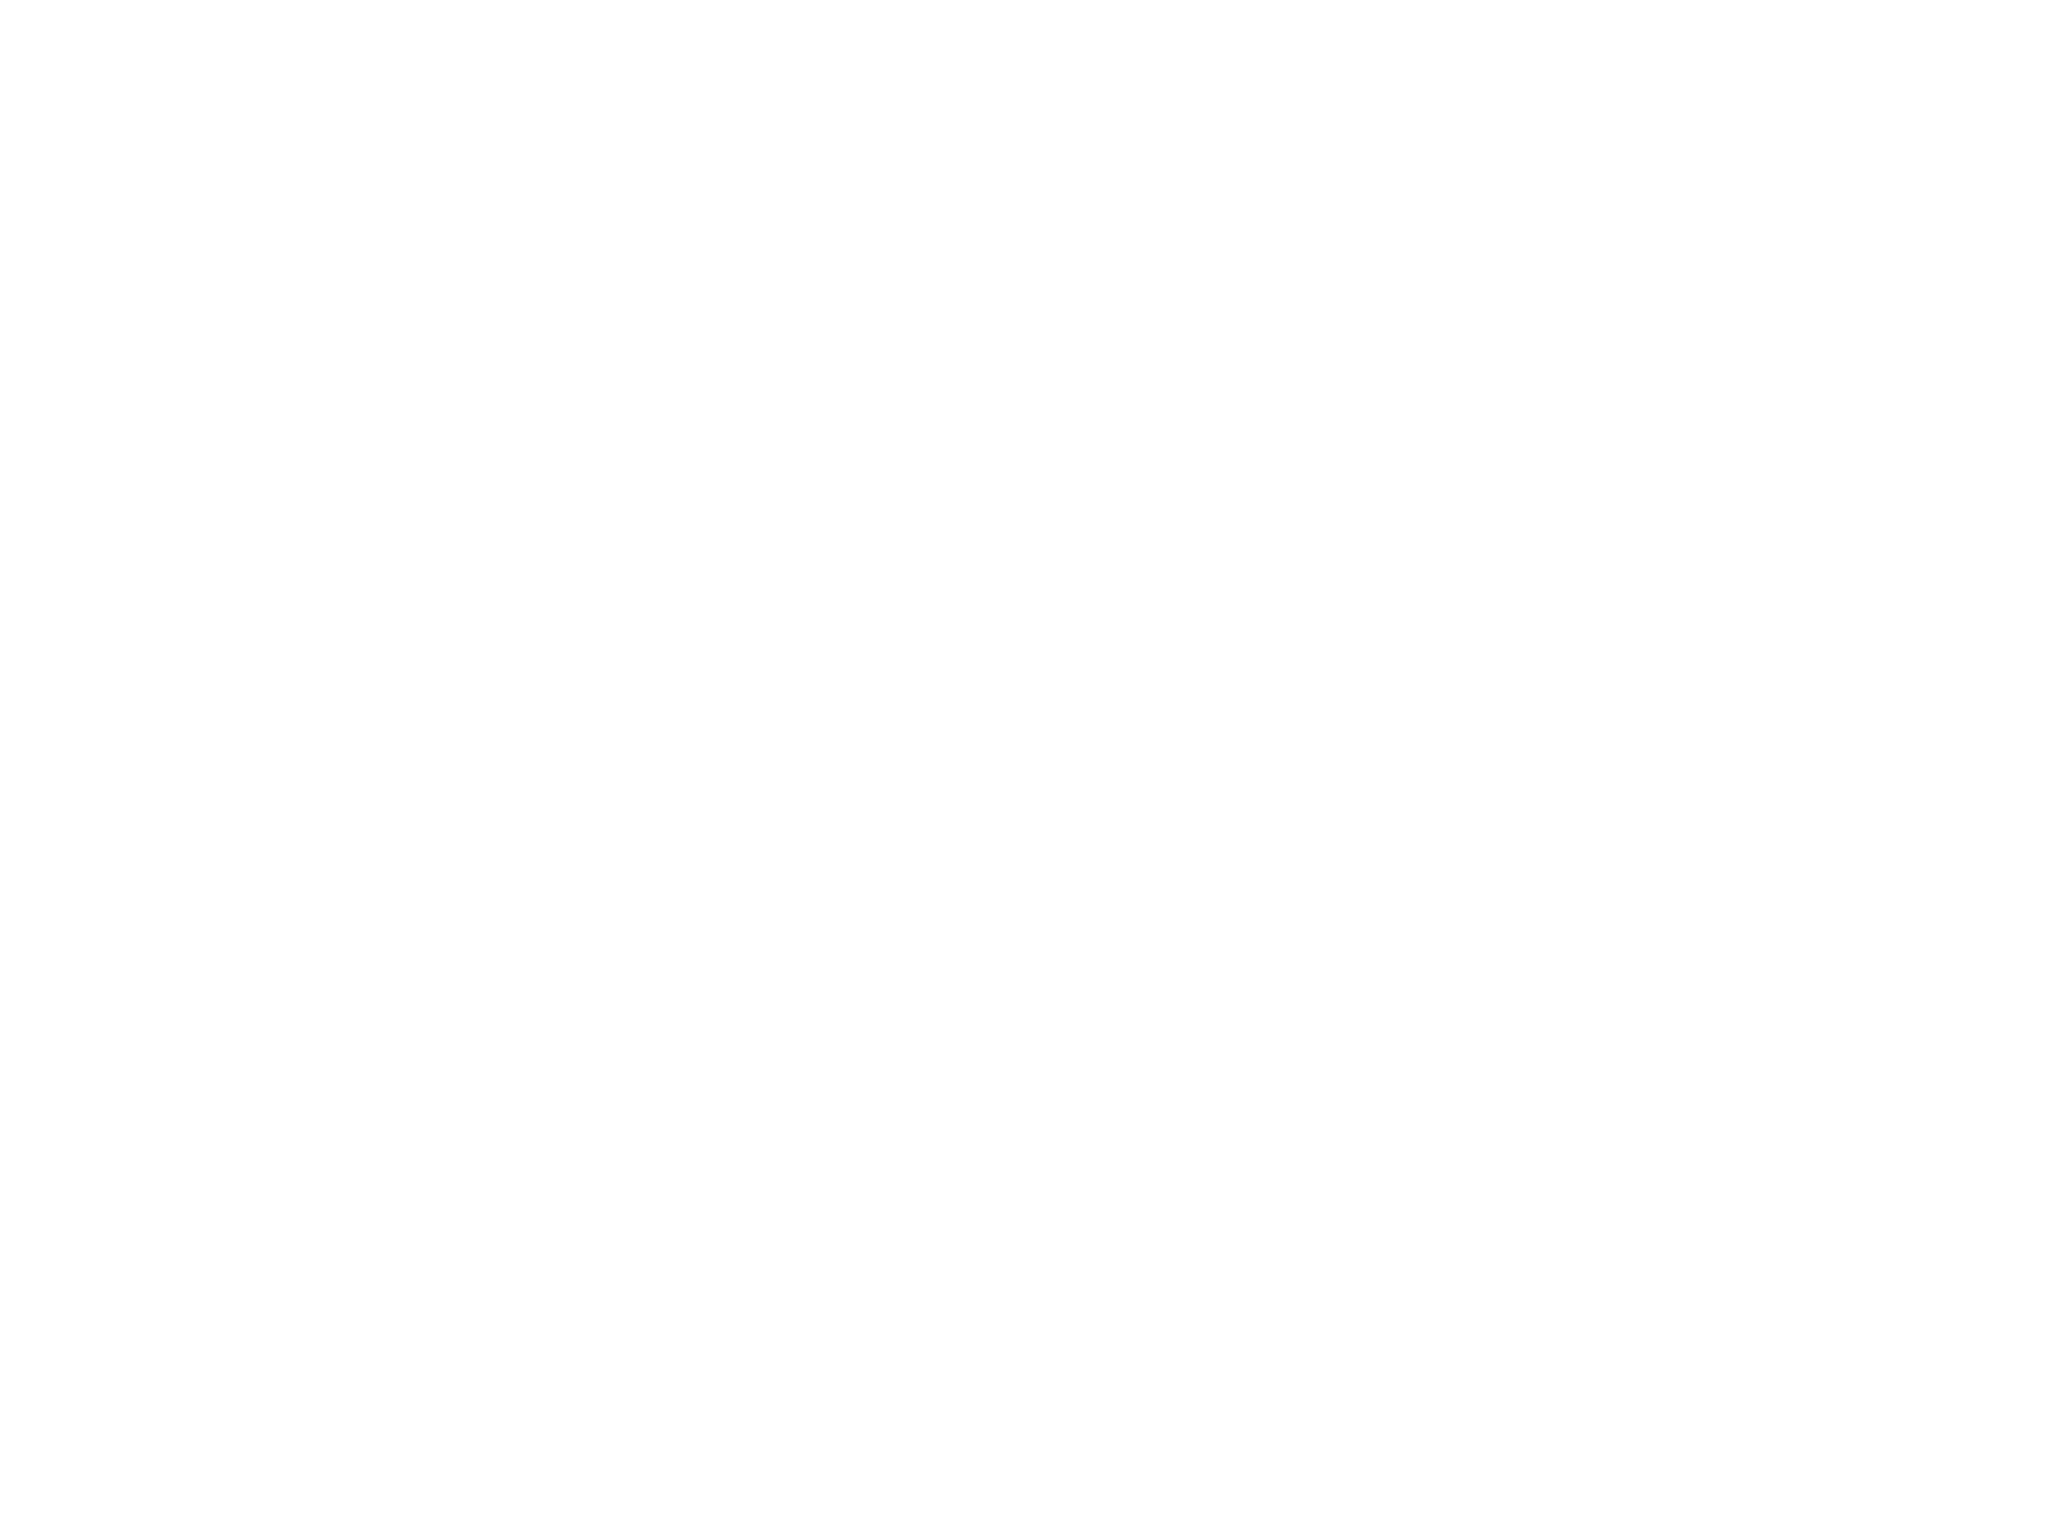
\includegraphics[width=0.3\textwidth]{img/sun} \\
    $p_{\bm{P} = \text{dry}} = 0.5$
    }
  &
  \makecell{
    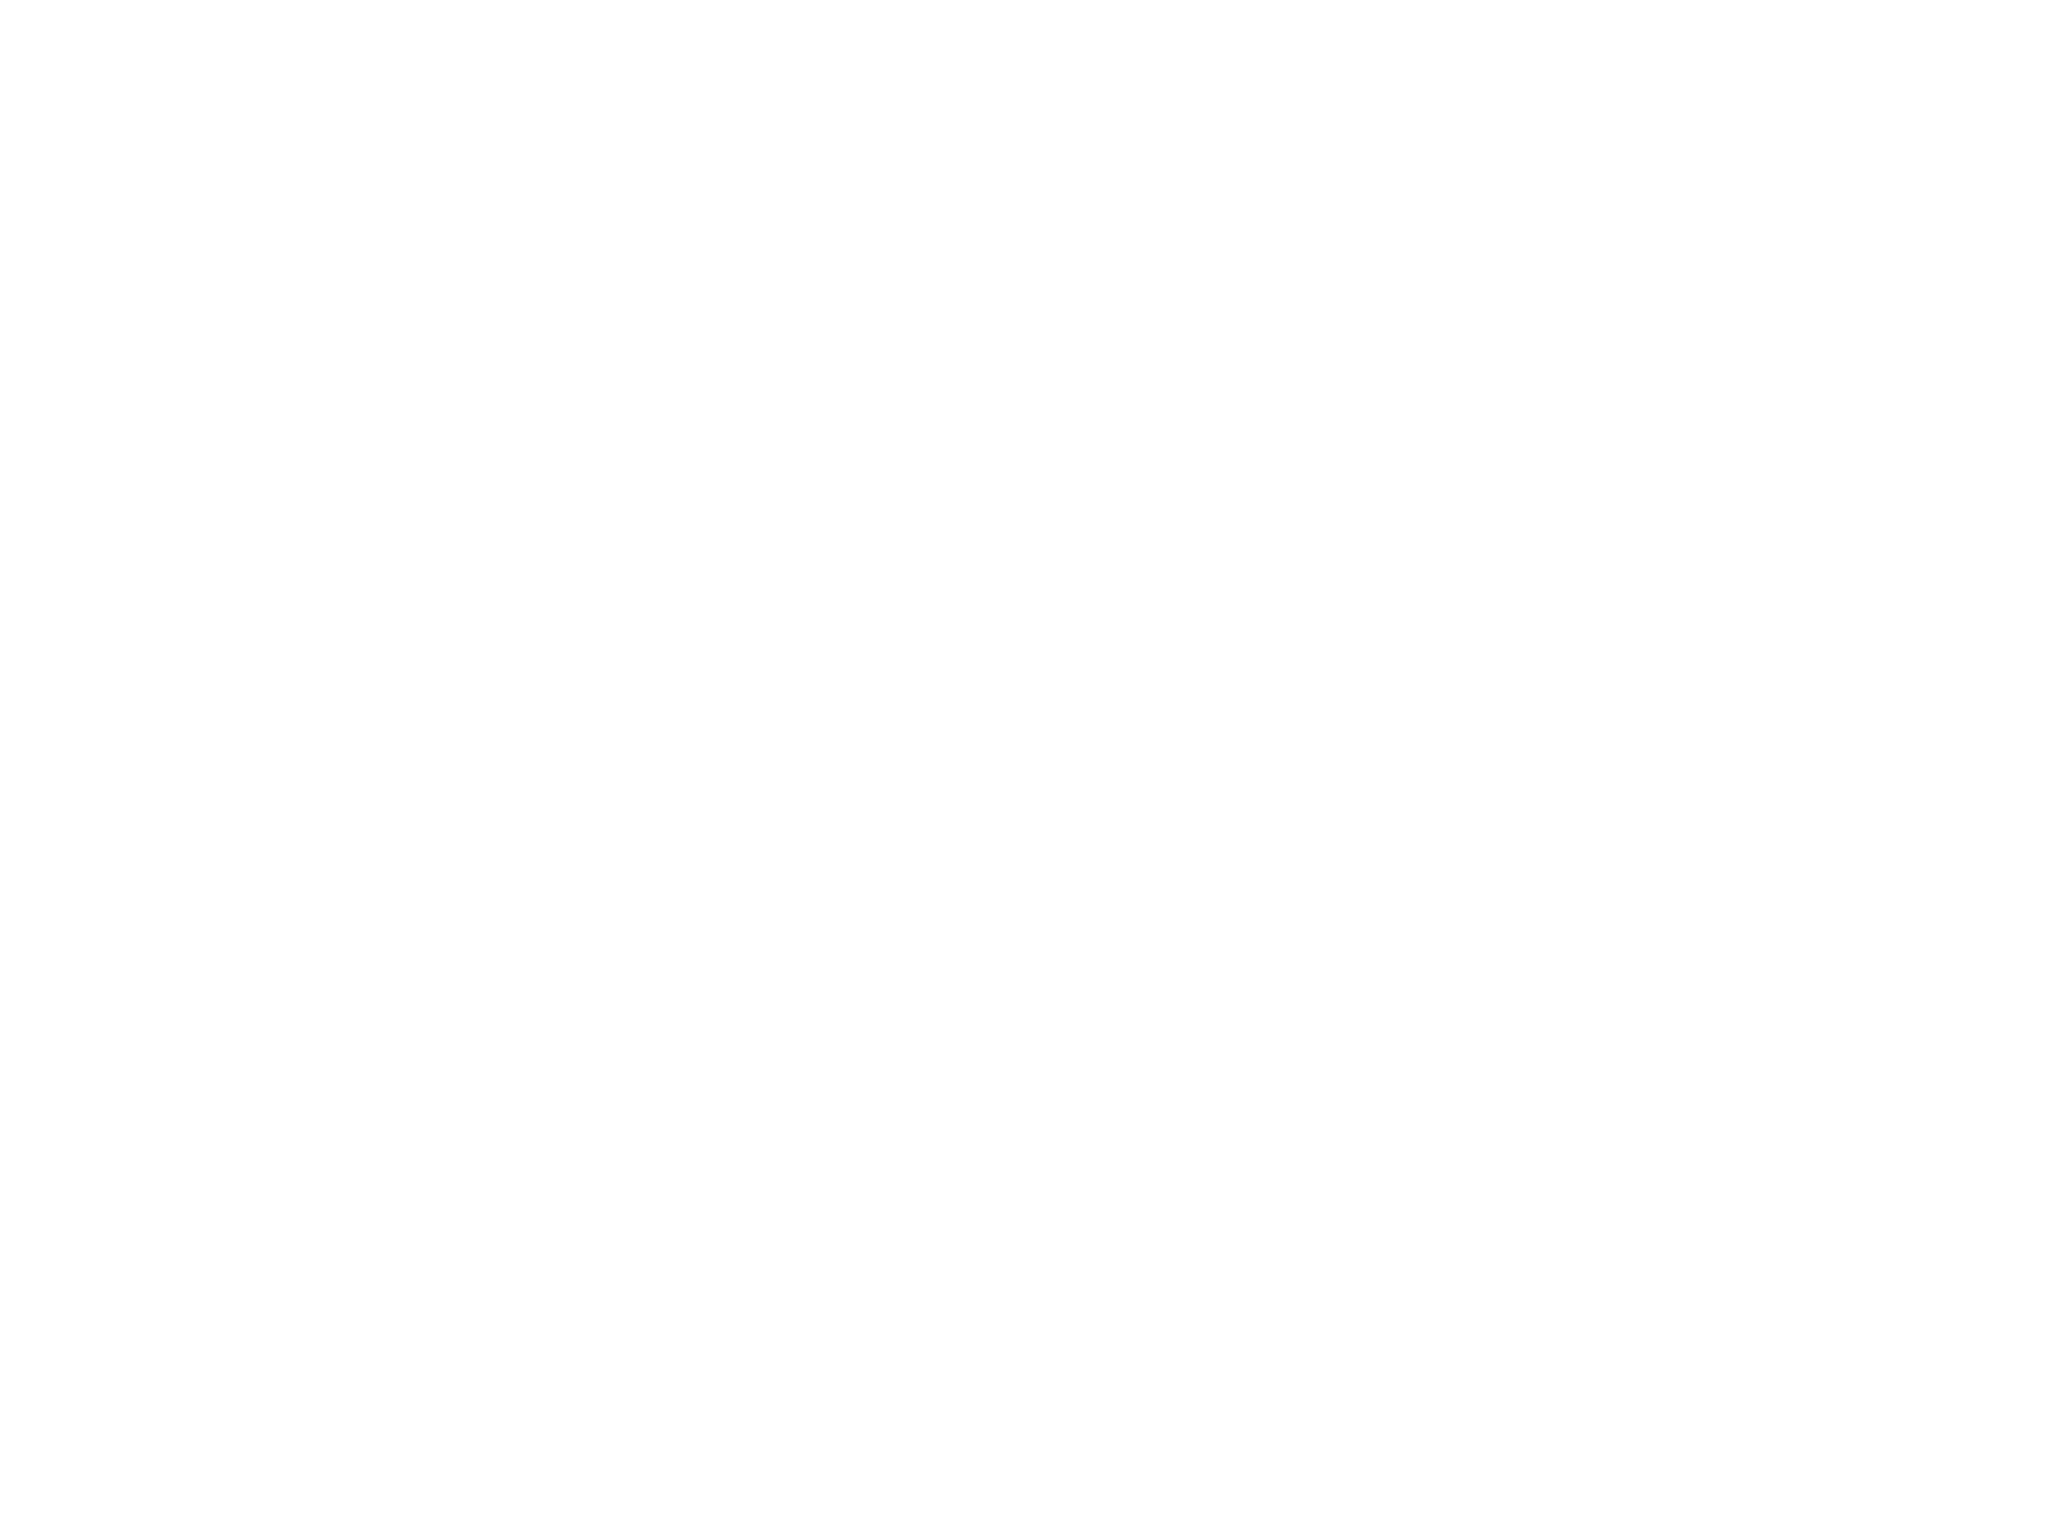
\includegraphics[width=0.3\textwidth]{img/cloud} \\
    $p_{\bm{P} = \text{wet}} = 0.5$
    }
  \end{tabular}
\end{center}

This setup looks familiar.
In the coin and die scenario, we had a pair of random variables that could each take on two values.
One random variable takes on each of its values with probability $\frac{1}{2}$.
the other random variable takes on one of its values with probability $\frac{9}{10}$ and the other with probability $\frac{1}{10}$.

The key difference is that precipitation and light are not independent.
Intuitively, we expect the wet and overcast conditions to be correlated and the dry and sunny conditions to be correlated.
For example, if it's raining we would be very surprised if it was sunny!

Let's look at how precipitation and light interact in our hypothetical scenario.
We will model the weather --- the combination of precipitation and light --- as a single random variable $\bm{W}$.
The weather can be in four possible states,
\begin{center}
 \begin{tabular}{c c || c | c }
 \multicolumn{2}{c}{\multirow{2}{*}{$\bm{W}$}} & \multicolumn{2}{c}{$\bm{P}$} \\
\multicolumn{2}{c}{} & rainy & dry \\ [0.5ex]
 \hline\hline
\multirow{10}{*}{$\bm{L}$} & sunny
& \makecell{
  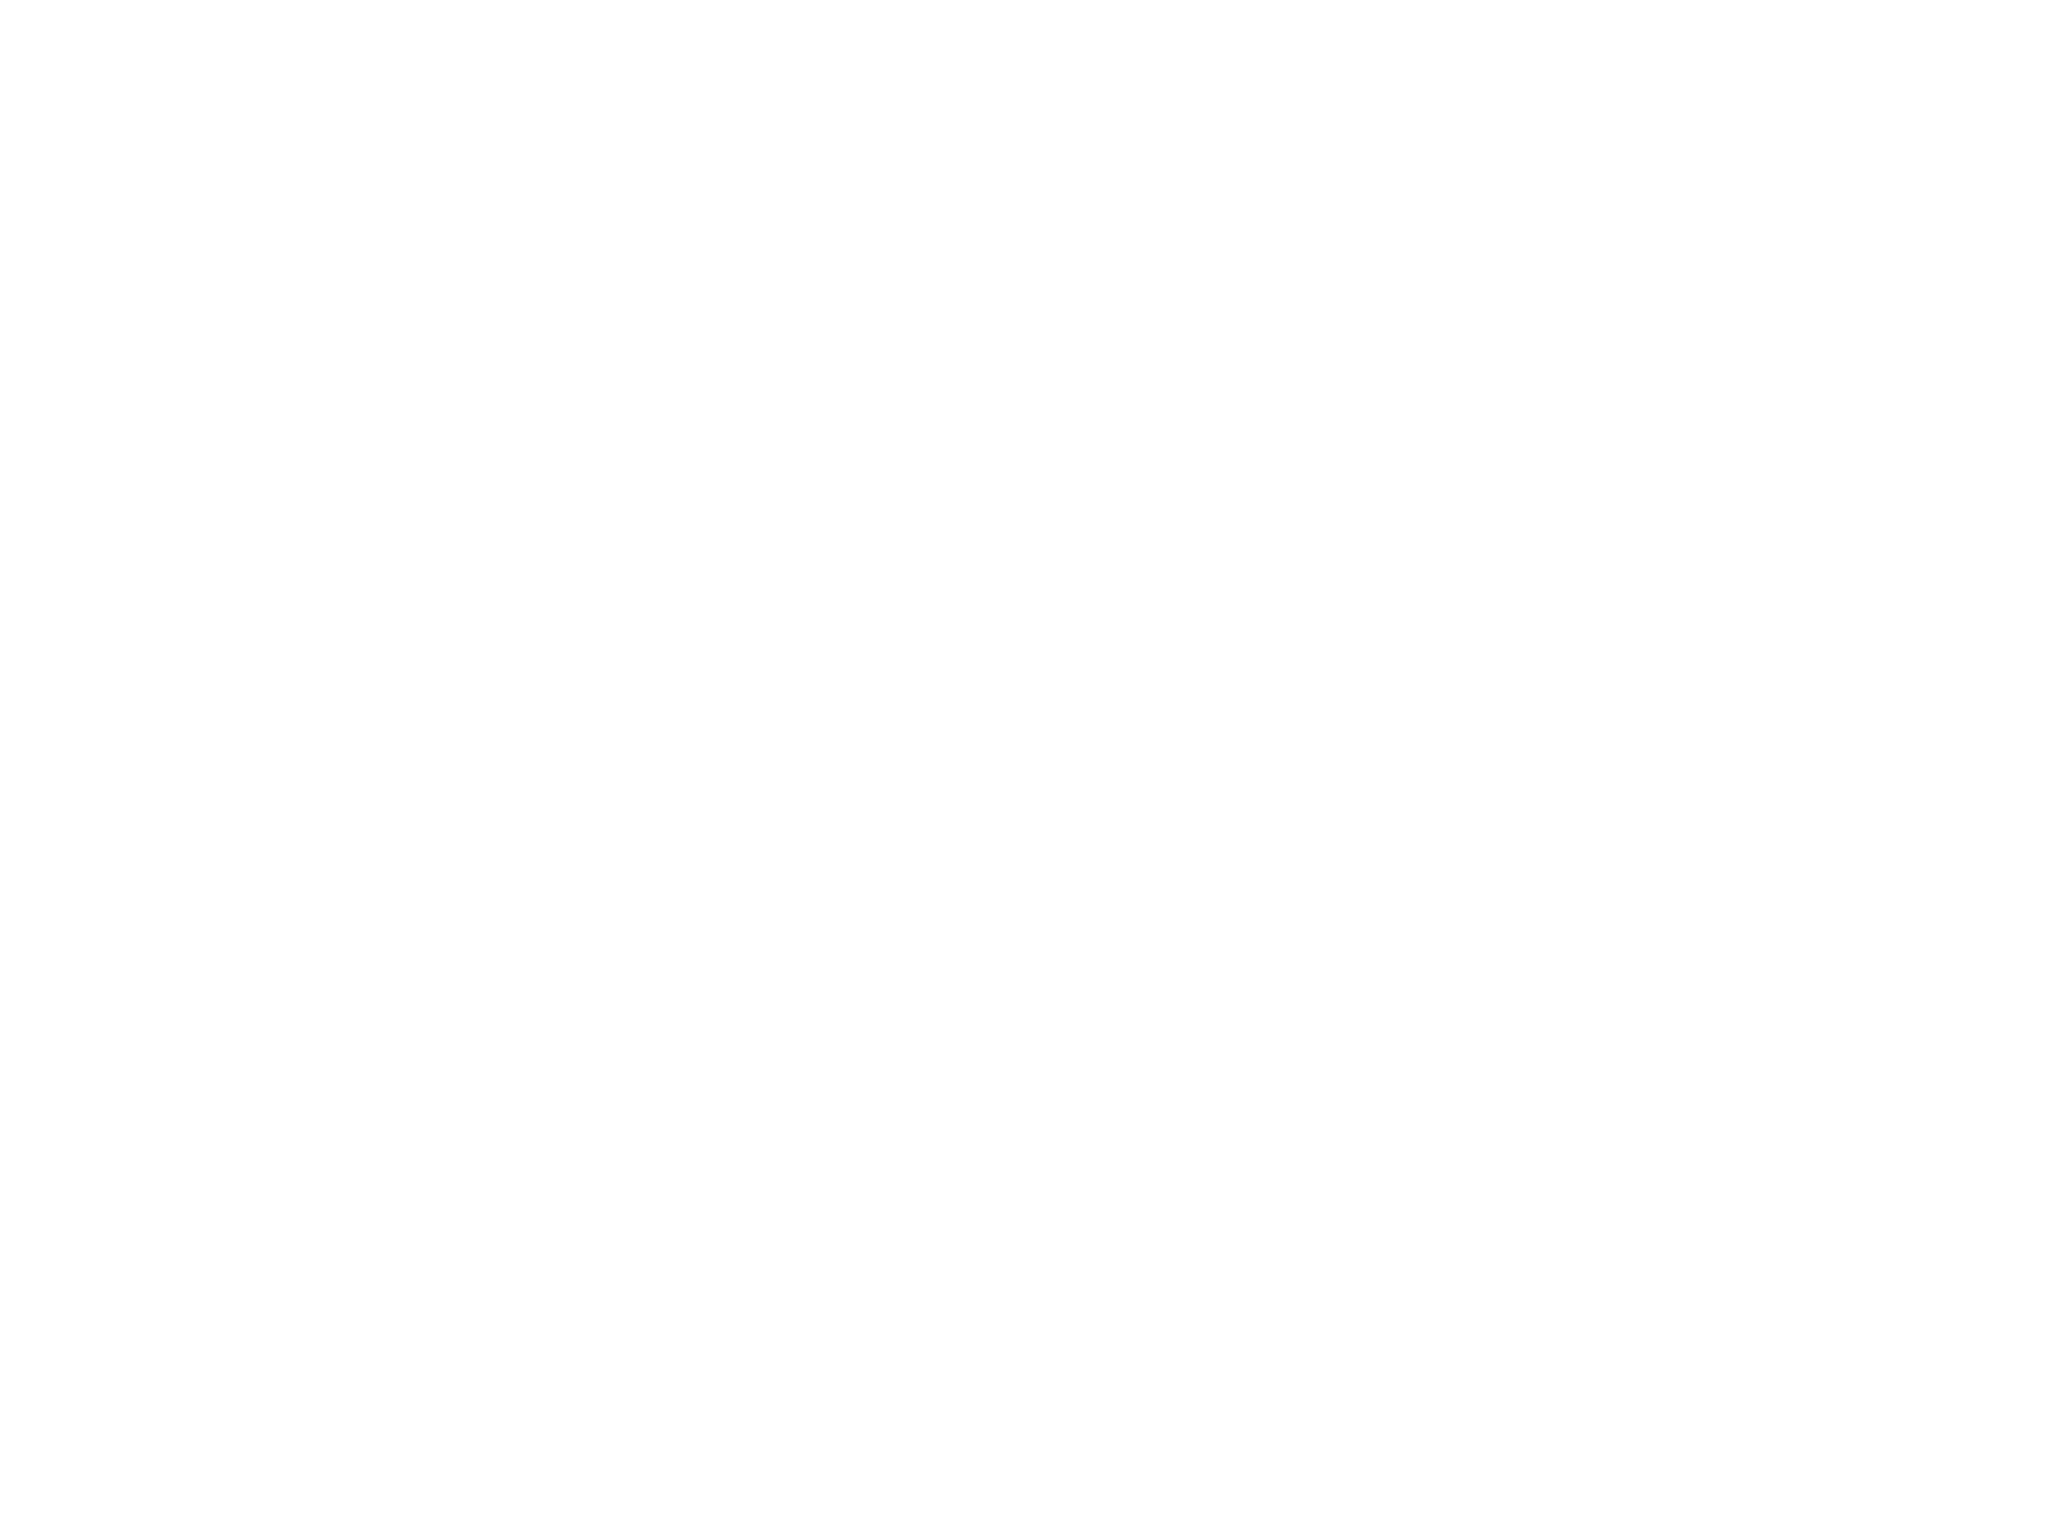
\includegraphics[trim= 0 0 0 0, clip, width=0.3\textwidth]{img/sun-rain} \\
  $\bm{W} = \text{``rainy, sunny''}$
  }
 & \makecell{
  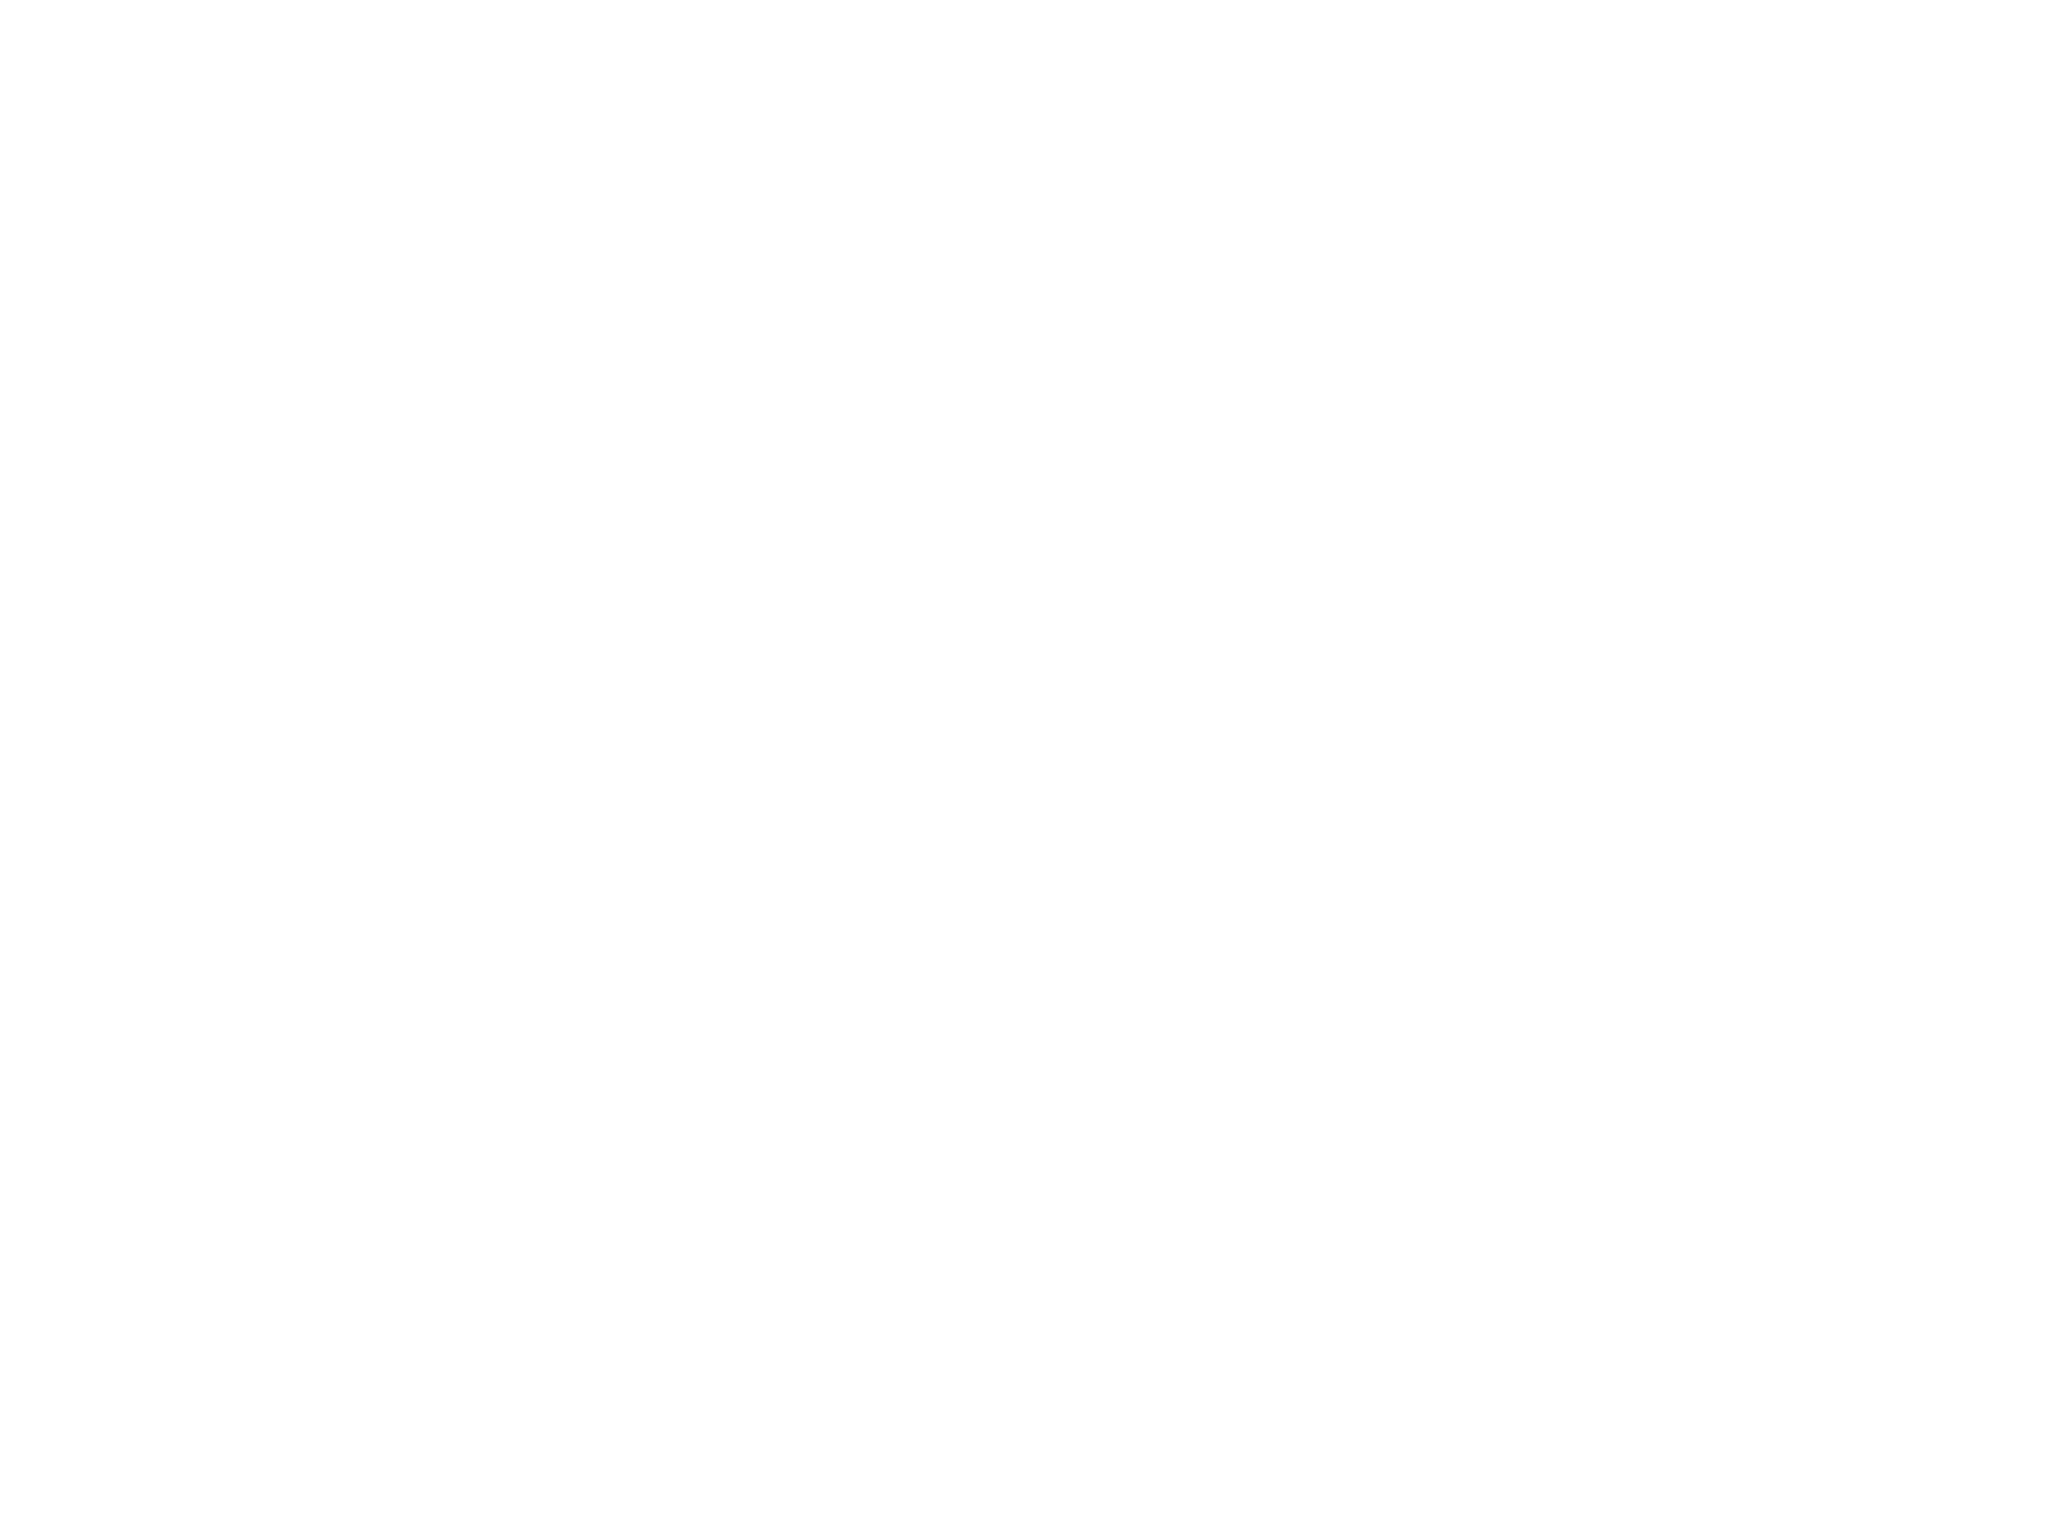
\includegraphics[trim= 0 0 0 0, clip, width=0.3\textwidth]{img/sun} \\
  $\bm{W} = \text{``dry, sunny''}$
  }
  \\
 \cline{2-4}
 & overcast
 & \makecell{
 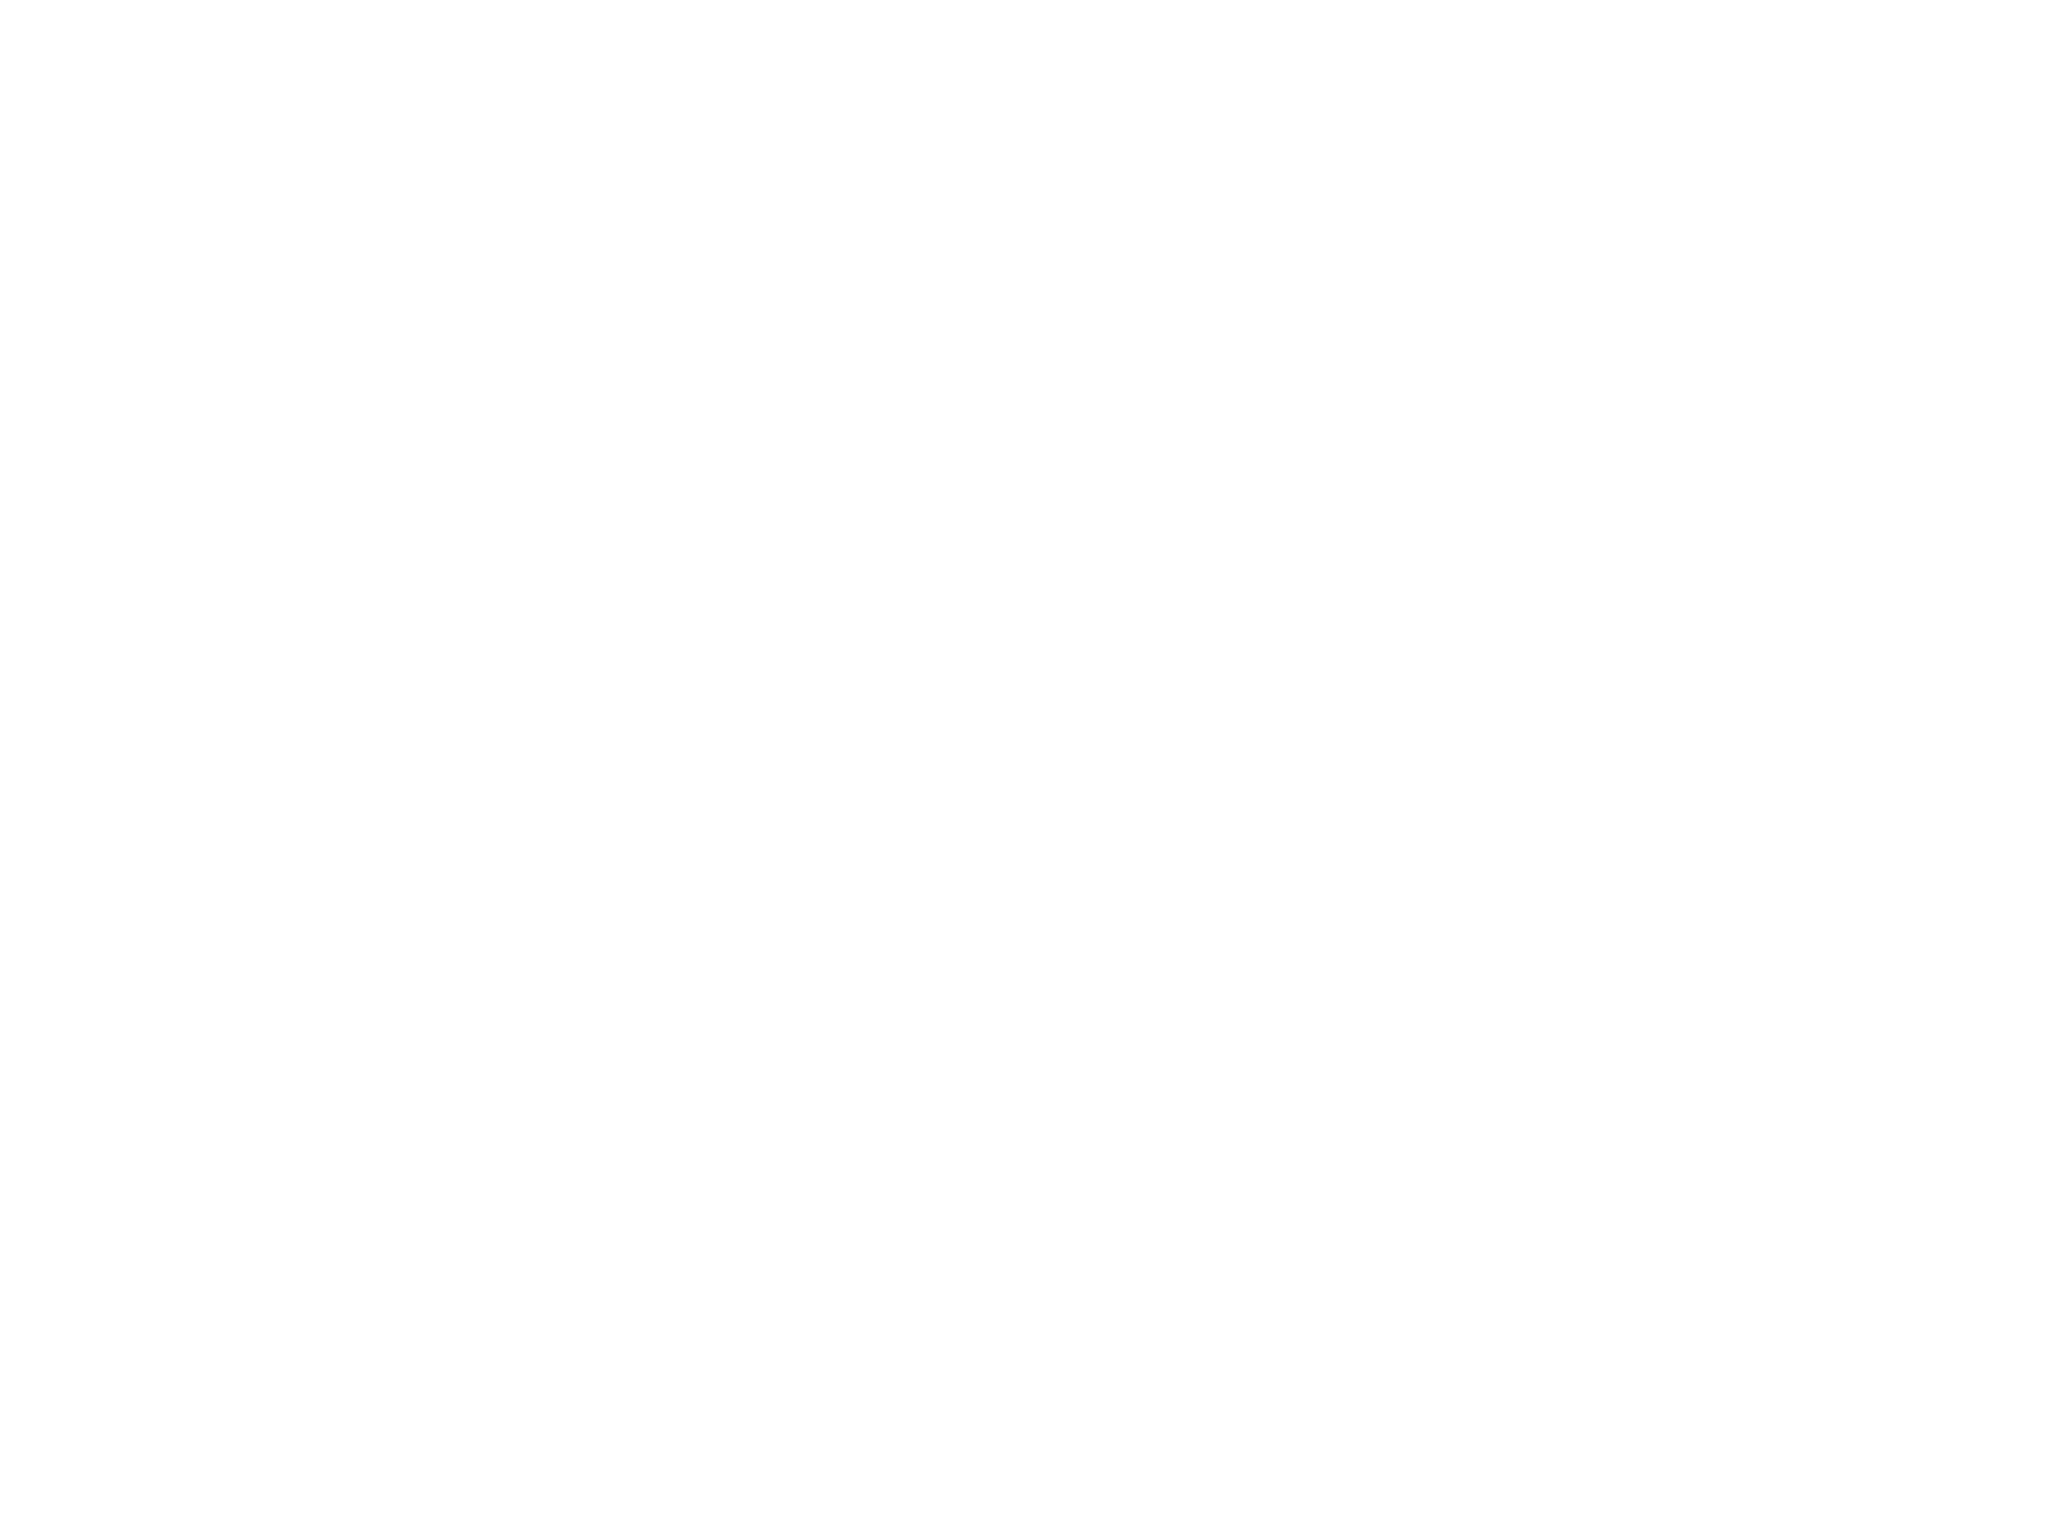
\includegraphics[trim= 0 0 0 0, clip, width=0.3\textwidth]{img/cloud-rain} \\
  $\bm{W} = \text{``rainy, overcast''}$}
 & \makecell{
 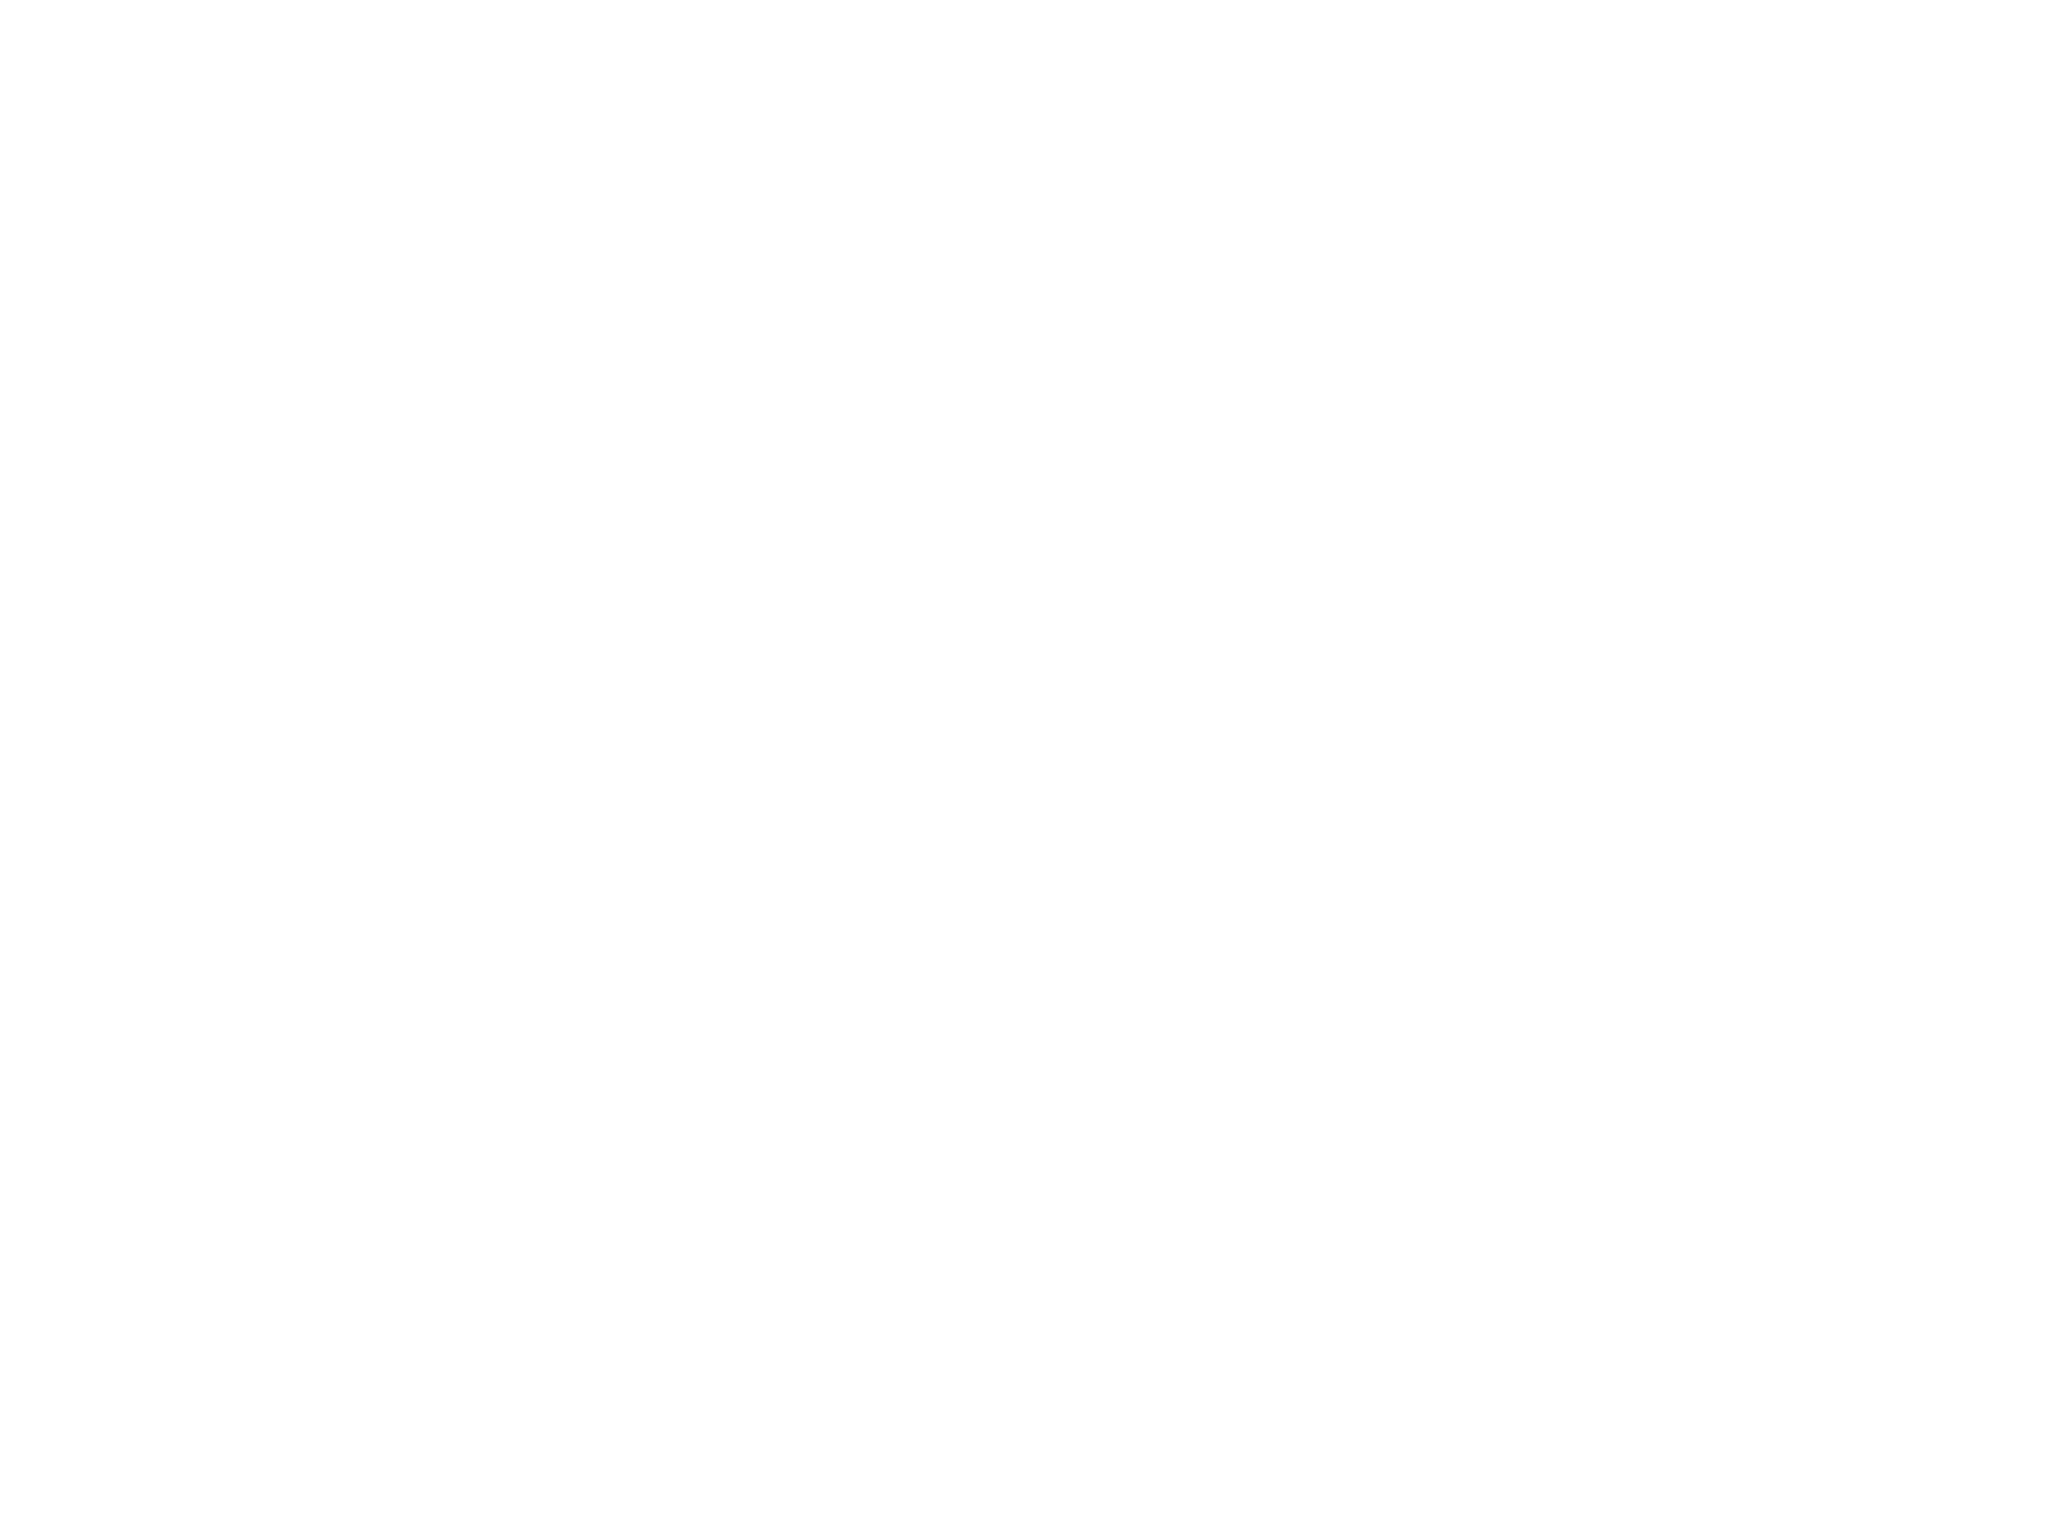
\includegraphics[trim= 0 0 0 0, clip, width=0.3\textwidth]{img/cloud} \\ $\bm{W} = \text{``dry, overcast''}$}
\end{tabular}
\end{center}

Because we are no longer operating under the assumption of independence, the probabilities of the four states of $\bm{W}$ can no longer be derived from the probability distributions of $\bm{P}$ (precipitation) and $\bm{L}$ (light).
Just as we took it at face value that in our scenario the probability of the sunny and cloudy condition are both $\frac{1}{2}$, we take the probability of each of the four possible states of $\bm{W}$ at face value as describing the particular scenario we are imagining.
(Of course, this is under the constraint that the marginal probabilities of $\bm{P}$ and $\bm{L}$ are consistent with what we stated before).
Let's define the probability distribution of $\bm{W}$ as follows,
\begin{center}
 \begin{tabular}{c c || c | c || c}
 \multicolumn{2}{c}{\multirow{2}{*}{$\bm{W}$}} & \multicolumn{2}{c}{$\bm{L}$} & {}\\
\multicolumn{2}{c}{} & sunny & overcast & sum \\ [0.5ex]
 \hline\hline
\multirow{2}{*}{$\bm{P}$} & wet & 0.005 & 0.095 & 0.1 \\
 \cline{2-5}
 & dry & 0.495 & 0.405 & 0.9 \\
 \hline\hline
  {} & sum & 0.5 & 0.5 & 1 \\ [1ex]
\end{tabular}.
\end{center}

The best way to get a feel for the distribution of $\bm{W}$ is to look at conditional probabilities.
For example, here's the probability that we observe the sunny weather given we know that it's wet outside,
\begin{align*}
P(\bm{L} = \text{sunny} | \bm{P} = \text{wet}) &= 0.05.
\end{align*}

Although we won't elaborate on it, calculating such conditional probabilities from the table above is very straightforward.
Let's look through the rest of the rest of the conditional probabilities we can calculate.

Consider
\begin{align*}
  P(\bm{L} = \text{sunny} | \bm{P} = \text{dry}) &= 0.55 \\
  P(\bm{L} = \text{sunny}) &= 0.5 \\
  P(\bm{L} = \text{sunny} | \bm{P} = \text{wet}) &= 0.05.
\end{align*}
Here, we see that the probability of observing sunny weather is greatest if we know that it's dry outside and very small if we know that it's wet outside.

Likewise,
\begin{align*}
P(\bm{L} = \text{overcast} | \bm{P} = \text{wet}) &= 0.95 \\
P(\bm{L} = \text{overcast}) &= 0.5 \\
P(\bm{L} = \text{overcast} | \bm{P} = \text{dry}) &= 0.45.
\end{align*}
The probability of observing overcast weather is greatest if we know that it's wet outside and less if we know that it's dry outside.

Similarly,
\begin{align*}
P(\bm{P} = \text{wet} | \bm{L} = \text{overcast}) &= 0.19 \\
P(\bm{P} = \text{wet}) &= 0.1 \\
P(\bm{P} = \text{wet} | \bm{L} = \text{sunny}) &= 0.01.
\end{align*}
The probability of observing wet weather is greatest if we know it's overcast outside and least if we know it's sunny outside.

Finally,
\begin{align*}
P(\bm{P} = \text{dry} | \bm{L} = \text{sunny}) &= 0.99 \\
P(\bm{P} = \text{dry}) &= 0.9 \\
P(\bm{P} = \text{dry} | \bm{L} = \text{overcast}) &= 0.81.
\end{align*}
The probability of observing dry weather is greatest if we know it's sunny outside and least if we know it's overcast.

Armed with a good understanding of the probability distribution of our weather $\bm{W}$, we're ready to talk entropy and information.
We can calculate entropy of a random variable whose distribution we know using Equation \ref{eqn:shannon}.
Let's do that for $\bm{W}$,
\begin{align*}
H(\textbf{light}) = 1
\end{align*}
for $\bm{L}$,

and, finally, for $\bm{P}$
\begin{align*}
TODO
\end{align*}

Similarly to the die and the coin, $S_{\text{light}} > S_{\text{precipitation}}$.

Here's the shocker,
\begin{align*}
H(\textbf{system A})
= - 0.005 \times \log_2(0.005)
+ - 0.095 \times \log_2(0.095)
+ - 0.495 \times \log_2(0.495)
+ - 0.405 \times \log_2(0.405)
\approx 1.391
\end{align*}

\begin{align*}
H(\textbf{light} | \textbf{precipitation})
+ P(\bm{P} = \text{wet}) \times H(\textbf{light} | \bm{P} = \text{wet})
+ P(\bm{P} = \text{dry}) \times H(\textbf{light} | \bm{P} = \text{dry})
= 0.1 \times [ - 0.05 \times \log_2(0.05) + - 0.95 \times \log_2(0.95) ]
+ 0.9 \times [ - 0.55 \times \log_2(0.55) + - 0.45 \times \log_2(0.45) ]
\approx 0.922
\end{align*}

\begin{align*}
I(\textbf{light} : \textbf{precipitation})
= H(\textbf{light}) - H(\textbf{light} | \textbf{precipitation})
\approx 1 - 0.922
\approx 0.078
\end{align*}

\begin{align*}
H(\textbf{precipitation} | \textbf{light})
= P(\bm{L} = \text{overcast}) \times H(\textbf{precipitation} | \bm{L} = \text{overcast})
+ P(\bm{L} = \text{sunny}) \times H(\textbf{precipitation} | \bm{L} = \text{sunny})
= 0.5 \times [ - 0.19 \times \log_2(0.19) + - 0.81 \times \log_2(0.81) ]
+ 0.5 \times [ - 0.01 \times \log_2(0.01) + - 0.99 \times \log_2(0.99) ]
\approx 0.391
\end{align*}

\begin{align*}
I(\textbf{precipitation} : \textbf{light})
= H(\textbf{precipitation}) - H(\textbf{precipitation} | \textbf{light})
\approx 0.469 - 0.391
\approx 0.078
\end{align*}

$0.78 \approx 0.78$,
so
\begin{align*}
I(\textbf{light} : \textbf{precipitation}) = I(\textbf{precipitation} : \textbf{light})
\end{align*}

note also,
\begin{align*}
H(\textbf{precipitation}) + H(\textbf{light}) - I(\textbf{light} : \textbf{precipitation})
= H(`System A`)
\end{align*}


% |       | \bm{L} = \text{sunny}    | \bm{L} = \text{overcast}  |          |
% | ----- | -------- | -------- | -------- |
% | \bm{P} = \text{wet} | 0.05     | 0.05     | sum: 0.1 |
% | \bm{P} = \text{dry} | 0.45     | 0.45     | sum: 0.9 |
% |       | sum: 0.5 | sum: 0.5 |          |
%
% H(`weather`)
% = - 0.05 \times \log_2(0.05)
% + - 0.05 \times \log_2(0.05)
% + - 0.45 \times \log_2(0.45)
% + - 0.45 \times \log_2(0.45)
% = - 0.1 \times \log_2(0.05)
% + - 0.9 \times \log_2(0.45)
% \approx 1.469
%
% H(\textbf{light}) + H(\textbf{precipitation})
% \approx 1 + 0.469
% \approx 1.469
% \approx H(`weather`)
%
% In this case,
% I(\textbf{precipitation} : \textbf{light})
% = I(\textbf{light} : \textbf{precipitation}) = 0.



\begin{center}

  \begin{tabular}{c | c | c | c || c}
   \multicolumn{4}{c}{\textbf{System A}} & {}\\
   sunny and wet & sunny and dry & overcast and wet & overcast and dry & sum \\ [0.5ex]
  \hline\hline
   0.05 & 0.45 & 0.05 & 0.45 & 1 \\ [1ex]
 \end{tabular}

\end{center}
